\section{Testing eBPF programs}\label{sec:testing}
The compiler features an end-to-end testing infrastructure to validate the 
correctness of a P4-eBPF/XDP program. The framework consists of a user space 
and a kernel testing pipeline, which run a test from the compilation 
until the actual runtime deployment of the program.

\subsection{Why Test in User-Space?}
Testing in user space isolates the specification of the eBPF/XDP program from 
the implementation. It is primarily intended to test the correctness of the
compiler and the generated C code without interference of the kernel verifier
and tooling. The user space testing framework does not depend on the 
LLVM~\cite{llvm} or any particular kernel version. It also does not require 
usage of \texttt{iproute2}~\cite{iproute} tooling such as \texttt{tc} or 
\texttt{ip}. 
Our goal is to ensure that a P4 program is functionally equivalent to its 
corresponding XDP C-code.

User space testing also guarantees debugging simplicity for the average
user. Tools such as GDB~\cite{gdb}, Valgrind~\cite{valgrind}, 
Wireshark~\cite{wireshark}, or plain statements
are readily available.



\begin{table*}[h]
	\begin{center}
		\begin{tabular}{|l|p{9cm}|} \hline
			\textbf{Command} & \textbf{Description} \\ \hline \hline
			\textbf{packet} port data & Insert a frame of bytes
			\textit{data} into port \textit{port}.    \\ \hline
			\textbf{expect} port data & Expect a frame of bytes
			\textit{data} on port \textit{port}.  \\ \hline
			\textbf{add} tbl priority match action & Insert a
			match-action entry with key \textit{match} and action
			\textit{action} into table \textit{tbl}. \\ \hline
			\textbf{setdefault} tbl action & Set the default action for table
			\textit{tbl}. \\
			\hline
			\textbf{check\_counter} tbl\_name key == n & Check if the value on
			the entry \textit{key} in counter table \textit{tbl} matches
			\textit{n}.  \\
			\hline
			\textbf{wait} & Pause any operation for a second. \\ \hline
		\end{tabular}
		\caption{The STF command palette.}\label{table:stf}
	\end{center}
\end{table*}

\subsection{The Simple Test Framework}
\begin{figure}
	\centering
	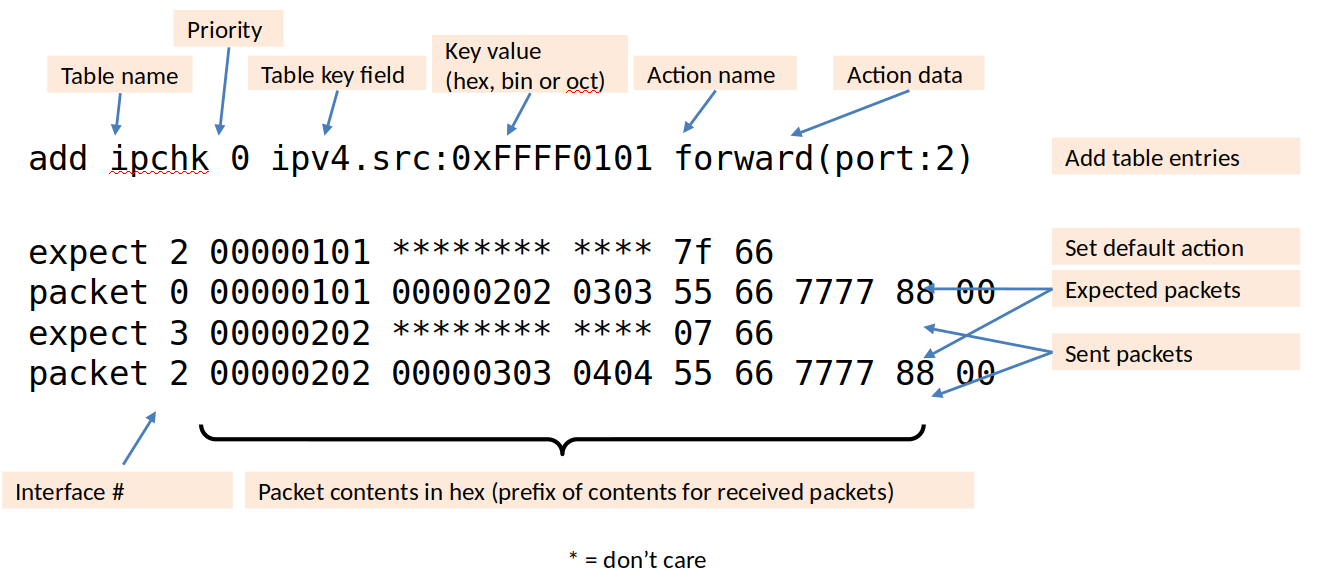
\includegraphics[width=\linewidth]{stf}
	\caption{Annotated example of a basic STF file.}
	\label{fig:stf}
\end{figure}
The simple test framework (STF) is a descriptive data-plane verification 
language. STF files define a set of actions which are intended to be 
sequentially executed on the data-plane.
While its original purpose is to assess switching and forwarding behavior, STF 
templates can also be used to test eBPF/XDP programs in isolation. 

An example STF action is \texttt{packet}. \texttt{packet} contains information 
about the byte content of an inbound Ethernet frame and the port which will 
receive it. Its counterpart, \texttt{expect}, defines where a given Ethernet 
frame is to be emitted. In a typical test case, we \textit{expect} our 
data-plane to forward a frame inserted by \texttt{packet} to a port specified 
by \texttt{expect}.
Another fundamental action in STF files is \texttt{add}, a simple PUT operation 
on data-plane tables. It describes which table to update and what key-value 
pair to insert.

The P4 compiler features a parser, which pre-processes the templates and 
generates an ordered command list. This list is interpreted by the eBPF testing 
framework, which produces capture files from the \texttt{packet} commands and 
converts \texttt{add} operations into eBPF map system calls.
Table \ref{table:stf} describes the full list of currently 
supported STF operations.

\paragraph{Example}
An example of an STF template can be seen in Figure \ref{fig:stf}. \texttt{add} 
defines that, if a packet's MAC source address matches with the 
key in table \texttt{macfwd}, we forward it to port 2. After the table update, 
the template instructs to insert packets on port 0 and 2 and to expect outputs 
on port 2 and 3.
The program operates correctly if a packet corresponding to the first input 
packet is emitted from port 3 (the default port) while the packet with the 
matching source address appears on port 2.

\begin{figure*}
	\centering
	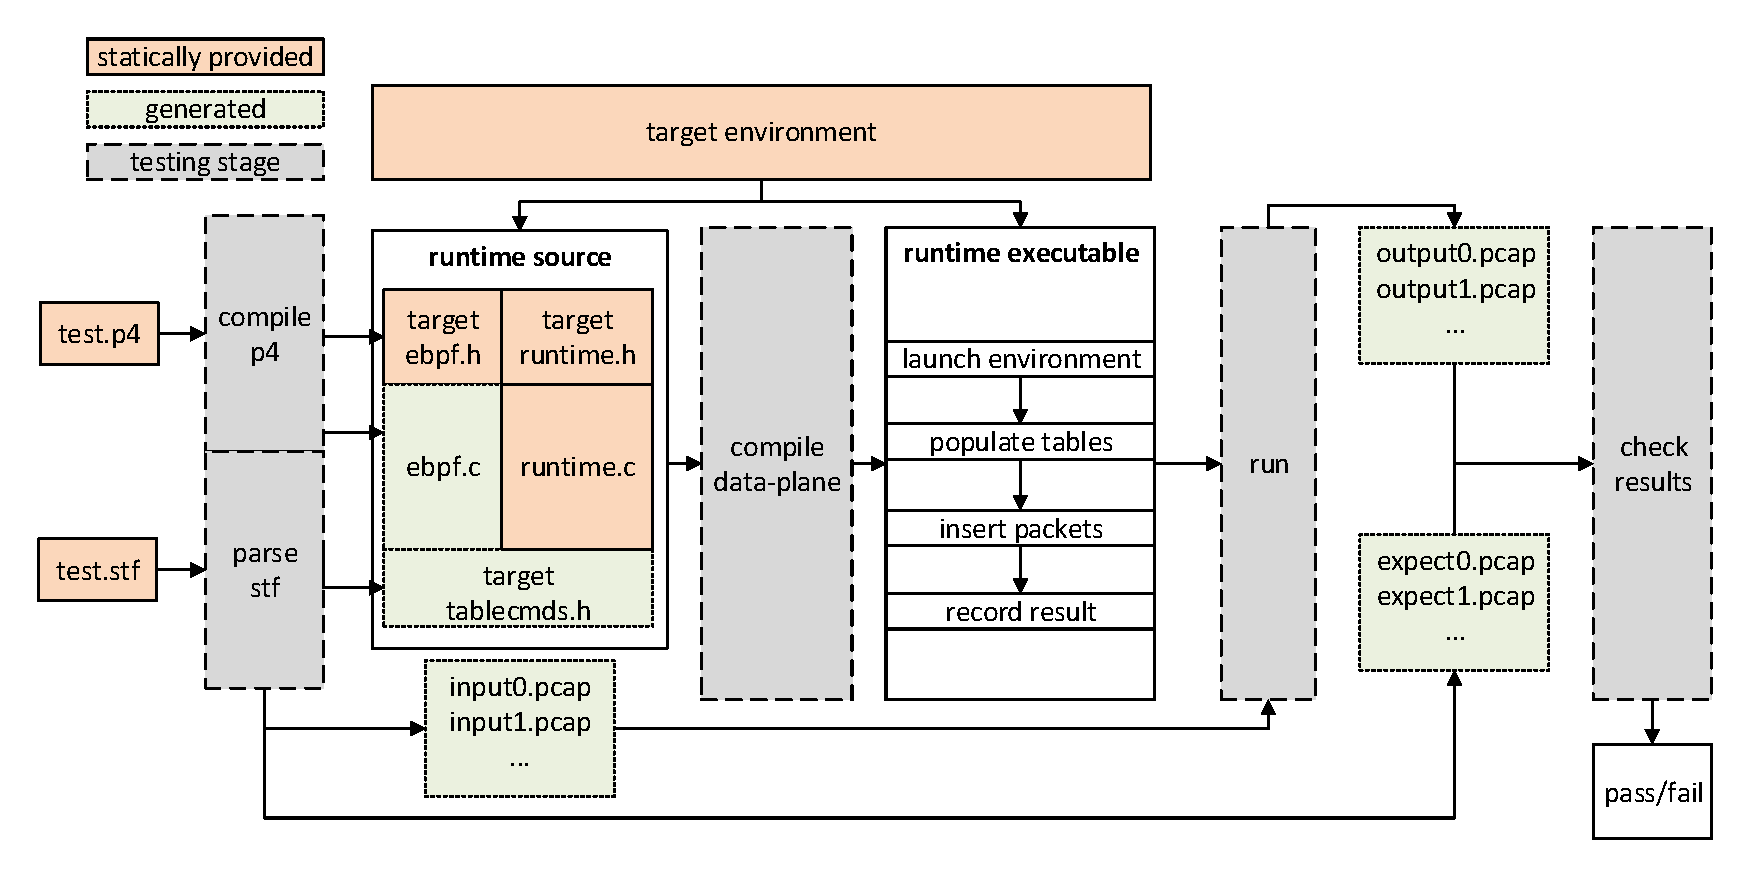
\includegraphics[width=\linewidth]{testing_workflow}
	\caption{Testing workflow for a P4-eBPF program. Environment and 
		target are provided by the user.}
	\label{fig:p4_testflow}
\end{figure*}

\subsection{The Test Runtime}
A P4-XDP test is an end-to-end verification of all stages of 
the compilation pipeline. This includes validation that the P4 code does 
compile, that the generated eBPF/XDP C is correct, and that the actual runtime 
behavior of the loaded program matches expectations.

\subsubsection{Architecture}
The test infrastructure is designed to be flexible as well as independent of 
the target backend. New testing frameworks can be added by creating a target 
file and linking it in the P4 test target folder. Each test will pass through 
five abstract test stages (see Figure \ref{fig:p4_testflow}):\\
\begin{enumerate}
\item\textbf{compile-p4:} Compile the P4 file to a data-plane binary.
\item \textbf{parse-stf:} Parse the stf file and interpret the output.
\item \textbf{compile-data-plane:} Load the P4 binary and create a runtime.
\item \textbf{run:} Start the runtime and insert the STF file inputs.
\item \textbf{check-results:} Compare the results with the STF 
expectations.
\end{enumerate}

The implementation of these stages is the responsibility of the compiler 
backend.
Currently, both kernel and user space eBPF/XDP targets are supported.

The user space testing framework defines a set of eBPF wrappers to approximate 
the kernel implementation. eBPF maps are implemented as hash maps, the 
userspace file descriptor operations are emulated by a shared in-memory 
registry. 
The functionality of the wrapper library is limited and only extends to the 
minimal eBPF map operations necessary for filtering and classifying.

Every target in the eBPF compiler is required to implement a custom 
\textit{target header}. This target header specifies how macros in the eBPF 
source file are expanded. For example, the header file \texttt{ebpf\_test.h} 
defines \texttt{BPF\_MAP\_LOOKUP\_ELEM} to call into the userspace registry 
whereas \texttt{ebpf\_kernel.h} defines it as the default eBPF system call.

\subsubsection{Running a Test}
A test requires only an STF template and a P4 program as input. The 
remaining files are generated or imported. The five testing stages are 
implemented as follows:

\paragraph{compile-p4}
Contingent on the target backend, the P4 program is compiled to either eBPF or 
to XDP C-Code. A header file containing all necessary includes accompanies the 
generated program. This stage confirms that the P4 file matches the expected 
syntax and describes valid P4 code.

\paragraph{parse-stf}
The framework parses the associated STF file and generates a set of input pcap 
files per port. The expected output packets are stored in a map for later use. 
In addition, all \texttt{add} operations are converted to eBPF map calls and 
exported as control file.

\paragraph{compile-data-plane}
Once the P4 and STF file have been parsed, the framework compiles 
the eBPF-C program, the eBPF wrappers, and the control-plane operations into a 
test runtime.

This runtime initializes all eBPF tables with entries specified by the STF 
file, then "runs" the data-plane by processing a set of input packets.
As input, the runtime takes a set of capture files, which are spliced into 
per-port lists and individually inserted into the datapath.
As the PcapNg~\cite{pcapng} format, which also contains port metadata, is 
not yet supported by libpcap, we associate the input port of a capture file with
its file name.

Along with the creation of the runtime, the kernel version compiles the 
eBPF/XDP program to an eBPF object using Clang and LLVM.

\paragraph{run}
At this point, the user and kernel frameworks diverge in behavior.

In the user space version, packets are converted to a mock \texttt{sk\_buff} 
structure and then directly passed into the to-be-tested eBPF/XDP function 
call. The output result is recorded and written to capture files on a per-port 
basis.

The kernel framework is intended to verify the correctness of an 
eBPF/XDP object in relation to the host kernel. This results in a more complex 
pipeline. 
Before the eBPF/XDP program is loaded, the framework creates a bridge running 
in an network namespace. Isolation via a namespace ensures that existing 
virtual interfaces and eBPF maps do not conflict with the test in question.
A number of virtual interfaces, corresponding to the highest port identifier in 
the STF file, are then attached to the bridge.
Once the virtual environment has been created, the compiled eBPF object is 
attached to all ports via \texttt{tc} (eBPF) or \texttt{ip} (XDP). If no STF 
file is present, the eBPF/XDP program is loaded directly into the bridge and 
the test completes.

Instead of directly calling into the eBPF program, the kernel runtime writes a 
packet to the associated port using raw sockets. The output 
results are recorded by attaching Tcpdump~\cite{tcpdump} to each interface.

\paragraph{check-results}
After the program has completed, the results are assembled and compared with 
the expected packets defined in the STF template. If the number of output 
packets or the dataframe content on a port does not match the specification, 
the test returns an error code and is marked as failed.

Both the user and kernel space runtime do not yet support testing for counters 
and table state. We have planned these extensions as future work.
